\subsection{Klassediagram}
For at illustrere modellaget i vores MVC-mønster, har vi produceret et klassediagram (se \myref{diagram:klassediagram} nedenfor) i UML, der simplificerer strukturen.
Det skal bemærkes, at klasserne og felterne er på dansk i diagrammet, og på engelsk i selve koden af programmet. \fxfatal{Der er ingen adgangsting på dette, private, protected, public etc. Er det bevist? Derudover er det ikke klart hvilken datatype hvert felt er, også om det er en liste eller ej. - Troels - Fikser figuren senere - Søren}

\begin{figure}[H]
\centering
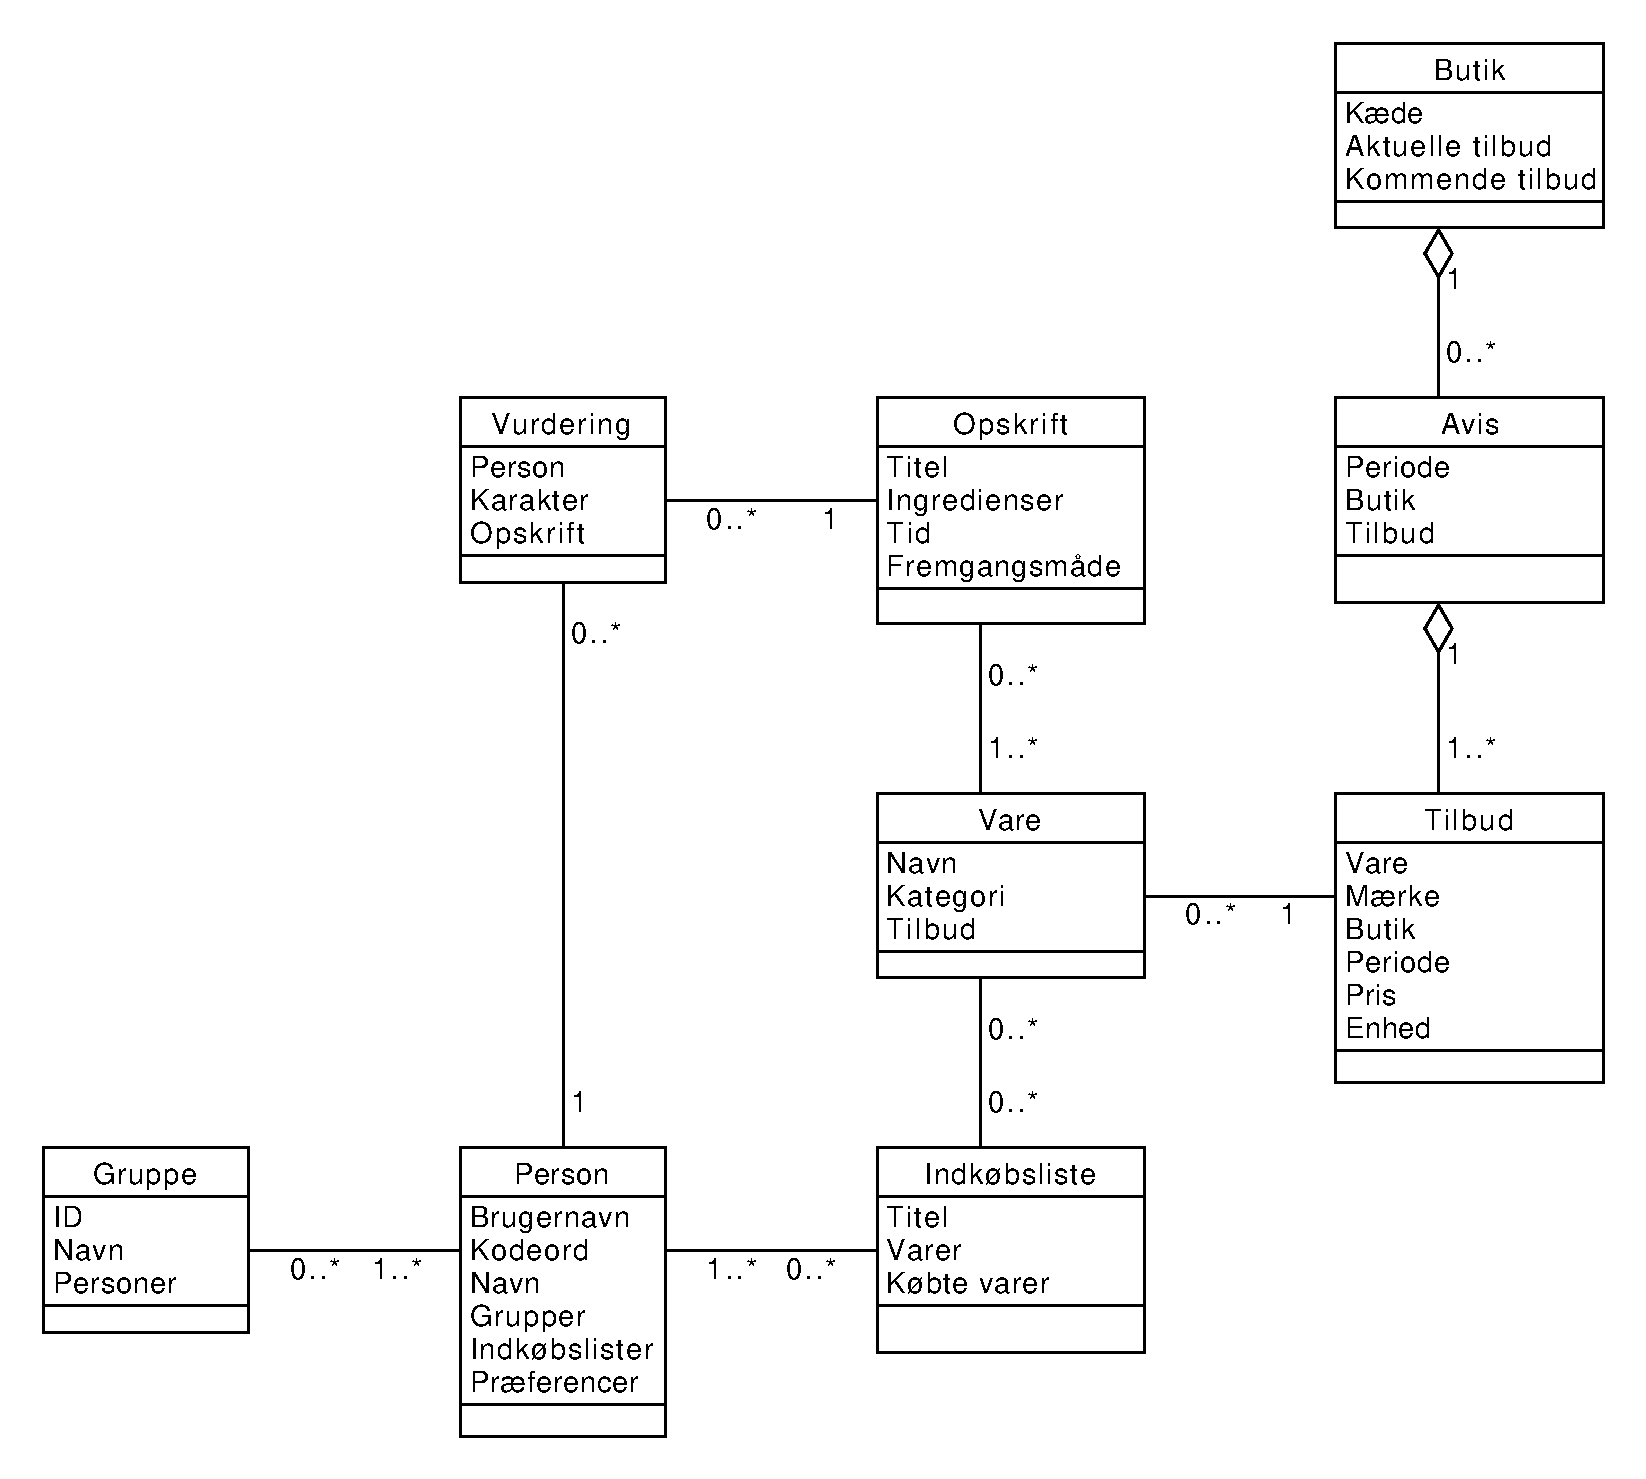
\includegraphics[width=0.8\linewidth]{/Diagrams/klassediagram_model_expanded_implemented.pdf}
\caption{UML klassediagram for modellaget i MVC-mønsteret}\label{diagram:klassediagram}
\end{figure}

\subsection{Klasserne}
Vi vil gennemgå klasserne, der optræder i klassediagrammet, og beskrive deres relationer samt deres felter.

\fxnote{Indsæt figur for hver enkelt klasse.}

\subsubsection{Person}
Person-klassen i modellen, er den der holder styr på brugeren og dennes basale attributter - herunder brugernavn, kodeord og kaldenavn.
Ydermere er det vigtigt, at objektet kan indeholde informationer om personens madpræferencer og vurderinger af opskrifter; dette er med til at give person-klassen en mere intim vinkel, og så at sige bedre afspejle den virkelige person, samt fungere som grundlag for anbefaling af opskrifter.
Det er naturligvis også vigtigt for et program, der omhandler bl.a. indkøbslister, at holde styr på en persons indkøbslister og lignende.
Til dette har person-klassen to felter der hedder henholdsvis, grupper og indkøbslister.
Begge felter er lister\fxfatal{Som nævnt tidligere er dette ikke klart fra diagrammet. - Troels}, der holder styr på personens relationer til netop grupper og indkøbslister - En person kan altså have relationer til flere grupper og flere indkøbslister, hvilket også kan ses ud fra de indtegnede relationer i klassediagrammet.


\subsubsection{Indkøbsliste}
Indkøbslister repræsenteres i systemet som klassen ´´Indkøbsliste'', og indeholder ID, titel og to lister med varer.
ID'et garanterer, at alle indkøbslister er unikke og kan skelnes fra hinanden på systemsiden.
Indkøbsliste-klassen har et titel felt, så brugeren også kan navigere mellem forskellige instanser.
De to lister af varer, holder styr på henholdsvis; varer som bliver tilføjet til listen, og varer som har været tilføjet men er blevet markeret som købt.
Der er således kun styr på ''overstregede'' varer - altså dem der er købt, og ikke varer som bliver slettet fra listen.
En indkøbsliste kan godt eksisterer uden varer, idet brugeren skal kunne oprette lister, inden der er taget stilling til, hvilke varer der skal bruges.
Indkøbsliste har kun relation til en gruppe, men kan godt have relationer til flere personer.\fxnote{Findes der stadig to lister - Bruger vi dem ?}

\subsubsection{Vare}
Vare-klassen indeholder tre felter: Et navn på varen, som er generisk, for eksempel ''Letmælk'' og ''Cola'' istedet for ''Arla Letmælk'' og ''Pepsi''; en kategori, der beskriver varen, for eksempel ''Mejeri'' eller ''Pålæg''; og en liste over tilbud, der holder styr på, hvis og hvor varen eventuelt er på tilbud.
En vare behøver ikke være på en indkøbsliste eller opskrift for at eksistere, og kan have relationer til nul til mange tilbud.

\subsubsection{Tilbud}
Et tilbud som instans af Tilbud-klassen, indeholder felter der beskriver: Varen, mærket, hvilken butik tilbuddet befinder sig i, hvilken periode tilbuddet gælder i, prisen på tilbudet, og hvilken enhed/mængde tilbudet er i.
Ud fra disse attributter er det muligt at identificere tilbudet, og brugeren kan tage stilling til, om det er relevant.


\subsubsection{Opskrifter}
\lipsum[1]

\subsubsection{Vurdering}
\lipsum[1]
